%!TEX program = xelatex

\documentclass[a4paper, openany, oneside]{memoir}
\usepackage[no-math]{fontspec}
\usepackage{pgfplots}
\pgfplotsset{compat=newest}
\usepackage{commath}
\usepackage{mathtools}
\usepackage{amssymb}
\usepackage{amsthm}
\usepackage{booktabs}
\usepackage{mathtools}
\usepackage{xcolor}
\usepackage[separate-uncertainty=true, per-mode=symbol]{siunitx}
\usepackage[noabbrev, capitalize]{cleveref}
\usepackage{listings}
\usepackage[american inductor, european resistor]{circuitikz}
\usepackage{amsmath}
\usepackage{amsfonts}
\usepackage{ifxetex}
\usepackage[dutch,english]{babel}
\usepackage[backend=bibtexu,texencoding=utf8,bibencoding=utf8,style=ieee,sortlocale=en_GB,language=auto]{biblatex}
\usepackage[strict,autostyle]{csquotes}
\usepackage{parskip}
\usepackage{import}
\usepackage{standalone}
\usepackage{hyperref}
%\usepackage[toc,title,titletoc]{appendix}

\ifxetex{} % Fonts laden in het geval dat je met Xetex compiled
    \usepackage{fontspec}
    \defaultfontfeatures{Ligatures=TeX} % To support LaTeX quoting style
    \setromanfont{Palatino Linotype} % Tover ergens in Font mapje in root.
    \setmonofont{Source Code Pro}
\else % Terug val in standaard pdflatex tool chain. Geen ondersteuning voor OTT fonts
    \usepackage[T1]{fontenc}
    \usepackage[utf8]{inputenc}
\fi
\newcommand{\references}[1]{\begin{flushright}{#1}\end{flushright}}
\renewcommand{\vec}[1]{\boldsymbol{\mathbf{#1}}}
\newcommand{\uvec}[1]{\boldsymbol{\hat{\vec{#1}}}}
\newcommand{\mat}[1]{\boldsymbol{\mathbf{#1}}}
\newcommand{\fasor}[1]{\boldsymbol{\tilde{\vec{#1}}}}
\newcommand{\cmplx}[0]{\mathrm{j}}
\renewcommand{\Re}[0]{\operatorname{Re}}
\newcommand{\Cov}{\operatorname{Cov}}
\newcommand{\Var}{\operatorname{Var}}
\newcommand{\proj}{\operatorname{proj}}
\newcommand{\Perp}{\operatorname{perp}}
\newcommand{\col}{\operatorname{col}}
\newcommand{\rect}{\operatorname{rect}}
\newcommand{\sinc}{\operatorname{sinc}}
\newcommand{\IT}{\operatorname{IT}}
\newcommand{\F}{\mathcal{F}}

\newtheorem{definition}{Definition}
\newtheorem{theorem}{Theorem}


\DeclareSIUnit{\voltampere}{VA} %apparent power
\DeclareSIUnit{\pii}{\ensuremath{\pi}}

\hypersetup{%setup hyperlinks
    colorlinks,
    citecolor=black,
    filecolor=black,
    linkcolor=black,
    urlcolor=black
}

% Example boxes
\usepackage{fancybox}
\usepackage{framed}
\usepackage{adjustbox}
\newenvironment{simpages}%
{\AtBeginEnvironment{itemize}{\parskip=0pt\parsep=0pt\partopsep=0pt}
\def\FrameCommand{\fboxsep=.5\FrameSep\shadowbox}\MakeFramed{\FrameRestore}}%
{\endMakeFramed}

% Impulse train
\DeclareFontFamily{U}{wncy}{}
\DeclareFontShape{U}{wncy}{m}{n}{<->wncyr10}{}
\DeclareSymbolFont{mcy}{U}{wncy}{m}{n}
\DeclareMathSymbol{\Sha}{\mathord}{mcy}{"58}
\addbibresource{../../includes/bibliography.bib}

\begin{document}

\section{Introduction}

\cref{cha:sampling,cha:reconstruction,cha:sampling_methods,cha:detection} have analysed and described several
sampling, reconstruction and detection techniques. It is in this chapter that we will evaluate their performance such that a discussion and a conclusion can be draw based on the specifications as described \cref{sec:theory-specs}. This chapter will start with an overview of the complete system, to continue with a description of the tests performed to assess the performance of this system. This chapter will end with the results
of those tests which will be discussed in \textbf{verwijs naar discussie chapter}.

\section{Overview}
A block diagram of the complete system is depicted in \cref{fig:theoretical_overview_system}. Considered options that did not make it into
the final system are grayed out. 

\begin{figure}[H]
\centering
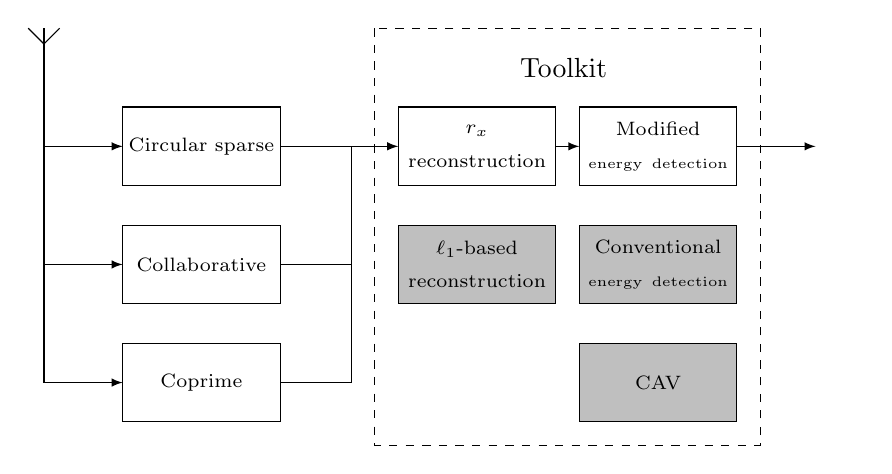
\begin{tikzpicture}
\draw  (-2,3) rectangle (0,2) node[pos=.5]{\scriptsize Circular sparse};
\draw  (-2,1.5) rectangle (0,0.5) node[pos=.5]{\scriptsize Collaborative};
\draw  (-2,0) rectangle (0,-1) node[pos=.5]{\scriptsize Coprime};
\draw  (1.5,3) rectangle (3.5,2) node[text width=5cm, align=center,pos=.5]{\scriptsize $r_x$\\ reconstruction};
% \draw  [fill=lightgray] (1.5,0) rectangle (3.5,-1) node[text width=5cm, align=center,pos=.5]{\scriptsize $r_x$\\ reconstruction};
\draw  [fill=lightgray](1.5,1.5) rectangle (3.5,0.5) node[text width=5cm, align=center,pos=.5]{\scriptsize $\ell_1$-based\\ reconstruction};
\draw  (3.8,3) rectangle (5.8,2) node[text width=5cm, align=center,pos=.5]{\scriptsize Modified\\\tiny energy detection};
\draw  [fill=lightgray] (3.8,1.5) rectangle (5.8,0.5) node[text width=5cm, align=center,pos=.5]{\scriptsize Conventional\\\tiny energy detection};
\draw  [fill=lightgray](3.8,0) rectangle (5.8,-1) node[pos=.5]{\scriptsize CAV};
\draw  [dashed] (1.2,4) rectangle (6.1,-1.3);
\node at (3.6,3.5) {Toolkit};
\draw [>=latex,->] (3.5,2.5) -- (3.8,2.5);
\draw [>=latex,->] (5.8,2.5) -- (6.8,2.5);
\draw [>=latex,->] (0,2.5) -- (1.5,2.5);
\draw [>=latex,->] (-3,2.5) -- (-2,2.5);
\draw [>=latex,->] (-3,1) -- (-2,1);
\draw [>=latex,->] (-3,-0.5) -- (-2,-0.5);
\draw (0,-0.5) -- (0.9,-0.5);
\draw (0,1) -- (0.9,1);
\draw (-3,-0.5) -- (-3,4);
\draw (0.9,-0.5) -- (0.9,2.5);
\draw (-2.8,4) -- (-3,3.8);
\draw (-3.2,4) -- (-3,3.8);
\node at (3.5,3) {};
\end{tikzpicture}
\caption{System overview with design choices}
\label{fig:theoretical_overview_system}
\end{figure}

\section{Testing}
To evaluate the performance of our system we will we use an artificial testing signal to test both the reconstructor and the detector.
Details on this signal generation can be found in \cref{ssec:test_signal}.

\subsection{Test signal}\label{ssec:test_signal}
To construct the testing signal given a desired SNR we take the following steps:

\begin{enumerate}
	\item Generate the signal $s[n]$ which is done by generating circular symmetric complex gaussian noise and filtering it such that it represents a bandpass signal with $-0.4\pi \leq \Omega \leq 0.4\pi$. The average power of the signal at frequencies in the passband is chosen such
	that the required SNR will be met. 
	\item Generate the additive circular symmetric complex gaussian noise signal $w[n]$ 
	\item Add $s[n]$ to $w[n]$ to produce the testing signal $x[n]$
\end{enumerate}



\subsection{Tests}
There are four parameters of the system, circled in \cref{tkz:test_system}, that will be used in our tests to asses the performance of the system:
\begin{enumerate}
	\item SNR of the input signal.
	\item The sampler type used to sample the input signal.
	\item The false alarm probability $p\ss{fa}$ of the detector.
\end{enumerate}

\begin{figure}[H]
\centering
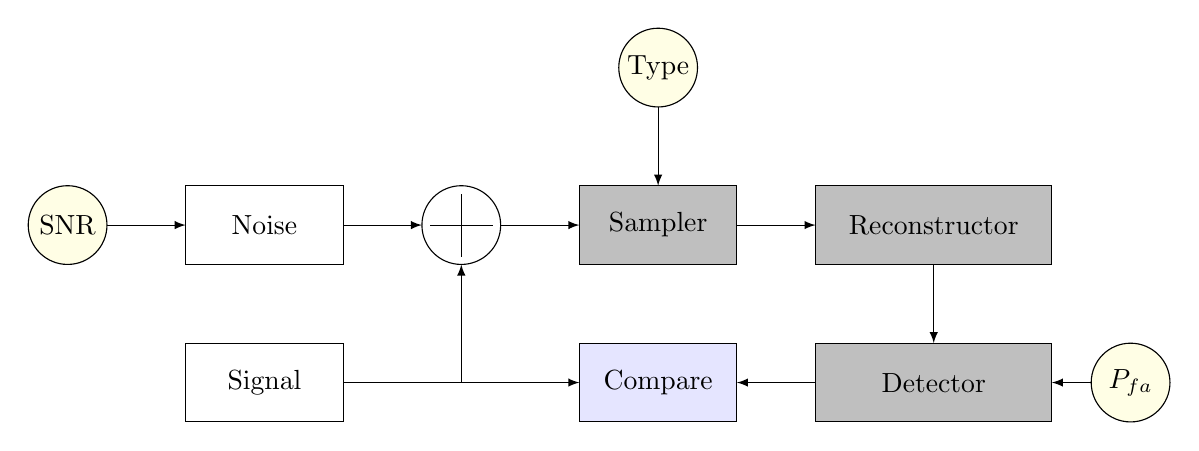
\begin{tikzpicture}

\draw  (-2,3.5) rectangle (0,2.5) node[pos=.5]{Noise};
\draw  (-2,1.5) rectangle (0,0.5) node[pos=.5]{Signal};
\draw  (1.5,3) ellipse (.5 and .5);
\draw  [fill=lightgray](3,3.5) rectangle (5,2.5) node[pos=.5]{Sampler};
\draw  [fill=lightgray](6,3.5) rectangle (9,2.5) node[pos=.5]{Reconstructor};
\draw  [fill=lightgray](6,1.5) rectangle (9,0.5) node[pos=.5]{Detector};
\draw  [fill=blue, opacity=.1](3,1.5) rectangle (5,0.5);
\draw  (3,1.5) rectangle (5,0.5)node[pos=.5]{Compare};



\draw (1.5,2.6) -- (1.5,3.4);
\draw (1.9,3) -- (1.1,3);
\draw [>=latex, ->] (0,3) -- (1,3);
\draw [>=latex, ->] (9.5,1) -- (9,1);
\draw [>=latex, ->] (4,4.5) -- (4,3.5);
\draw [>=latex, ->] (1.5,1) -- (1.5,2.5);
\draw [>=latex, ->] (-3,3) -- (-2,3);
\draw [>=latex, ->] (6,1) -- (5,1);
\draw [>=latex, ->] (0,1) -- (3,1);
\draw [>=latex, ->] (7.5,2.5) -- (7.5,1.5);
\draw [>=latex, ->] (2,3) -- (3,3);
\draw [>=latex, ->] (5,3) -- (6,3);


\draw   [fill=yellow, opacity=.1] (-3.5,3) ellipse (.5 and .5);
\draw   [fill=yellow, opacity=.1] (10,1) ellipse (.5 and .5);

\draw   [fill=yellow, opacity=.1] (4,5) ellipse (.5 and .5);

\draw   (-3.5,3) ellipse (.5 and .5) node{SNR};
\draw  (10,1) ellipse (.5 and .5) node{$P_{fa}$};

\draw  (4,5) ellipse (.5 and .5) node{Type};

\end{tikzpicture}
\caption{Testing the system}\label{tkz:test_system}
\end{figure}

Our tests will be targeted at
\begin{enumerate}
	\item adressing the performance of the reconstruction and feeding it an artificial constructed signal while
	\begin{enumerate}
		\item varying the sampling technique used to sample the signal (as described in \cref{cha:sampling_methods});
		\item varying the compression rate and the oversampling factor (as described in \cref{cha:reconstruction}).
	\end{enumerate}
	By comparing the reconstructed the power spectral density to the power spectral density recovered directly from the constructed test signal, we can evaluate the correctness of reconstruction when used with a specific sampling technique.
	Furthermore the dependence on the oversampling factor and the compression factor can be evaluated from those test results. 
	\item adressing the performance of detection on the reconstructed signal. The energy detector as described in \cref{ssec:ari_ed} will be evaluated by tests that make use of the test signal as described in \cref{ssec:test_signal}. 
	The detector is applied to the output of the reconstructor while	
	\begin{enumerate}
		\item varying the signal-to-noise ratio of the test signal; 
		\item varying the false alarm probability the detector 
		should allow;
		\item varying the compression rate of the reconstructor.
	\end{enumerate}
	Using these results we can construct the receiver operating characteristic curves (ROC-curves) which plot the detection probability versus the false alarm probability of the detector. From these curves the minimum signal strength and the detectors performance on a random signal can be evaluated. Furthermore the detection performance of the system as a whole can be evaluated by comparing these curves for different compression rates.
	\end{enumerate}

\section{Results}


%%%%%% PLOT: ALL SAMPLING METHODS
\begin{filecontents*}{plots/data-circ1.csv}
x, y
1.0000,-0.8677
2.0000,-0.9958
3.0000,-1.0846
4.0000,-1.1462
5.0000,-1.1877
6.0000,-1.2179
7.0000,-1.2525
8.0000,-1.2841
9.0000,-1.3028
10.0000,-1.3270
11.0000,-1.3476
12.0000,-1.3662
13.0000,-1.3878
14.0000,-1.4007
15.0000,-1.4189
16.0000,-1.4325
17.0000,-1.4488
18.0000,-1.4564
19.0000,-1.4604
20.0000,-1.4848
\end{filecontents*}

\begin{filecontents*}{plots/data-circ2.csv}
x, y
1.0000,-0.7942
2.0000,-0.9330
3.0000,-1.0226
4.0000,-1.0731
5.0000,-1.1180
6.0000,-1.1673
7.0000,-1.1904
8.0000,-1.2188
9.0000,-1.2412
10.0000,-1.2720
11.0000,-1.2944
12.0000,-1.3132
13.0000,-1.3161
14.0000,-1.3448
15.0000,-1.3515
16.0000,-1.3678
17.0000,-1.3865
18.0000,-1.3903
19.0000,-1.4067
20.0000,-1.4126
\end{filecontents*}

\begin{filecontents*}{plots/data-copr.csv}
x, y
1.0000,-0.8841
2.0000,-1.0174
3.0000,-1.0917
4.0000,-1.1523
5.0000,-1.1834
6.0000,-1.2243
7.0000,-1.2628
8.0000,-1.2902
9.0000,-1.3204
10.0000,-1.3418
11.0000,-1.3621
12.0000,-1.3806
13.0000,-1.3940
14.0000,-1.4147
15.0000,-1.4292
16.0000,-1.4482
17.0000,-1.4541
18.0000,-1.4630
19.0000,-1.4802
20.0000,-1.4862
\end{filecontents*}

\begin{filecontents*}{plots/data-collab.csv}
x, y
1.0000,-0.8541
2.0000,-0.9976
3.0000,-1.0853
4.0000,-1.1385
5.0000,-1.1811
6.0000,-1.2290
7.0000,-1.2528
8.0000,-1.2877
9.0000,-1.3010
10.0000,-1.3312
11.0000,-1.3490
12.0000,-1.3800
13.0000,-1.3855
14.0000,-1.4063
15.0000,-1.4289
16.0000,-1.4288
17.0000,-1.4461
18.0000,-1.4579
19.0000,-1.4730
20.0000,-1.4745
\end{filecontents*}

\begin{figure}
	\centering
	\begin{tikzpicture}
		\begin{axis}[
				xlabel={Sampling time (ms)},
				ylabel={$\log_{10}(\text{NMSE})$},
				width=11cm,
				height=8cm,
				scale=1,
				grid=both,
				axis lines=left,
				legend entries={Circular sparse sampling, Coprime sampling, Collorative sampling},
				legend cell align=left
			]
		    \addplot [
			    color=red,
			    solid,
			    mark=o
		    ] table [x=x, y=y, col sep=comma]{plots/data-circ1.csv};
		    % \addplot [
			   %  color=green,
			   %  solid,
			   %  mark=o
		    % ] table [x=x, y=y, col sep=comma]{plots/data-circ2.csv};
		    \addplot [
			    color=green,
			    solid,
			    mark=o
		    ] table [x=x, y=y, col sep=comma]{plots/data-copr.csv};
		    \addplot [
			    color=blue,
			    solid,
			    mark=o
		    ] table [x=x, y=y, col sep=comma]{plots/data-collab.csv};
		\end{axis}
	\end{tikzpicture}
	\caption{Normalised mean squared errors of the reconstructed power spectral densities by different sampling methods. The plot assumes a Nyquist frequency of \SI{25}{MHz}. The sampling techniques are described in \cref{tab:sampling-nmse}.}
	\label{fig:plot-nmse}
\end{figure}

\begin{table}
	\centering
	\begin{tabular}{llll}
		\textbf{Sampling technique} & \textbf{Compression} & \textbf{Configuration} & \textbf{Downsampling} \\ \hline
		Circular sparse ruler sampling & $31\%$ & $4$ samplers & $13 \times$ \\
		Coprime sampling & $45\%$ & $2$ samplers, periods $4T$ and $5T$ & $4 \times$ \\
		Collaborative & $46\%$ &$6$ samplers over $2$ devices & $13 \times$
	\end{tabular}
	\caption{Description of the sampling techniques depicted in \cref{fig:plot-nmse}}
	\label{tab:sampling-nmse}
\end{table}

%%%%%%


%%%%% PLOT: CIRCULAR
\begin{filecontents*}{plots/data-circ-N7.csv}
x, y
1.0000,-1.1552
2.0000,-1.3148
3.0000,-1.3921
4.0000,-1.4497
5.0000,-1.4765
6.0000,-1.5246
7.0000,-1.5701
8.0000,-1.6004
9.0000,-1.6108
10.0000,-1.6388
11.0000,-1.6494
12.0000,-1.6936
13.0000,-1.7016
14.0000,-1.7145
15.0000,-1.7207
16.0000,-1.7373
17.0000,-1.7628
18.0000,-1.7772
19.0000,-1.7917
20.0000,-1.7826
\end{filecontents*}

\begin{filecontents*}{plots/data-circ-N13.csv}
x, y
1.0000,-0.8544
2.0000,-0.9964
3.0000,-1.0845
4.0000,-1.1374
5.0000,-1.1829
6.0000,-1.2151
7.0000,-1.2324
8.0000,-1.2825
9.0000,-1.3114
10.0000,-1.3244
11.0000,-1.3541
12.0000,-1.3699
13.0000,-1.3847
14.0000,-1.4144
15.0000,-1.4383
16.0000,-1.4353
17.0000,-1.4413
18.0000,-1.4667
19.0000,-1.4701
20.0000,-1.4775
\end{filecontents*}

\begin{filecontents*}{plots/data-circ-N21.csv}
x, y
1.0000,-0.6490
2.0000,-0.7952
3.0000,-0.8770
4.0000,-0.9352
5.0000,-0.9736
6.0000,-1.0154
7.0000,-1.0399
8.0000,-1.0627
9.0000,-1.0926
10.0000,-1.1152
11.0000,-1.1273
12.0000,-1.1415
13.0000,-1.1596
14.0000,-1.1800
15.0000,-1.1915
16.0000,-1.2198
17.0000,-1.2260
18.0000,-1.2222
19.0000,-1.2500
20.0000,-1.2542
\end{filecontents*}

\begin{figure}
	\centering
	\begin{tikzpicture}
		\begin{axis}[
				xlabel={Sampling time (ms)},
				ylabel={$\log_{10}(\text{NMSE})$},
				width=11cm,
				height=8cm,
				scale=1,
				grid=both,
				axis lines=left,
				legend entries={$43\%$ compression, $31\%$ compression, $24\%$ compression},
				legend cell align=left
			]
		    \addplot [
			    color=red,
			    solid,
			    mark=o
		    ] table [x=x, y=y, col sep=comma]{plots/data-circ-N7.csv};
		    \addplot [
			    color=green,
			    solid,
			    mark=o
		    ] table [x=x, y=y, col sep=comma]{plots/data-circ-N13.csv};
		    \addplot [
			    color=blue,
			    solid,
			    mark=o
		    ] table [x=x, y=y, col sep=comma]{plots/data-circ-N21.csv};
		\end{axis}
	\end{tikzpicture}
	\caption{Normalised mean squared errors of the reconstructed power spectral densities by circular sparse sampling. The plot assumes a Nyquist frequency of \SI{25}{MHz}. The sampling techniques are described in \cref{tab:sampling-nmse-circ}.}
	\label{fig:plot-nmse-circ}
\end{figure}

\begin{table}
	\centering
	\begin{tabular}{llll}
		\textbf{Sampling technique} & \textbf{Compression} & \textbf{Configuration} & \textbf{Downsampling} \\ \hline
		Circular sparse ruler sampling & $43\%$ & $3$ samplers & $7 \times$ \\
		Circular sparse ruler sampling & $31\%$ & $4$ samplers & $13 \times$ \\
		Circular sparse ruler sampling & $24\%$ & $5$ samplers & $21 \times$ \\
	\end{tabular}
	\caption{Description of the sampling techniques depicted in \cref{fig:plot-nmse-circ}}
	\label{tab:sampling-nmse-circ}
\end{table}

%%%%%%%

%%%%%% PLOT: COPRIME

\begin{filecontents*}{plots/data-cop-35.csv}
x, y
1.0000,-1.0051
2.0000,-1.1439
3.0000,-1.2190
4.0000,-1.2912
5.0000,-1.3452
6.0000,-1.3798
7.0000,-1.3969
8.0000,-1.4345
9.0000,-1.4665
10.0000,-1.4877
11.0000,-1.5047
12.0000,-1.5283
13.0000,-1.5366
14.0000,-1.5412
15.0000,-1.5725
16.0000,-1.5946
17.0000,-1.5928
18.0000,-1.6110
19.0000,-1.6198
20.0000,-1.6315
\end{filecontents*}

\begin{filecontents*}{plots/data-cop-45.csv}
x, y
1.0000,-0.8841
2.0000,-1.0174
3.0000,-1.0917
4.0000,-1.1523
5.0000,-1.1834
6.0000,-1.2243
7.0000,-1.2628
8.0000,-1.2902
9.0000,-1.3204
10.0000,-1.3418
11.0000,-1.3621
12.0000,-1.3806
13.0000,-1.3940
14.0000,-1.4147
15.0000,-1.4292
16.0000,-1.4482
17.0000,-1.4541
18.0000,-1.4630
19.0000,-1.4802
20.0000,-1.4862
\end{filecontents*}

\begin{filecontents*}{plots/data-cop-47.csv}
x, y
1.0000,-0.7382
2.0000,-0.8825
3.0000,-0.9470
4.0000,-1.0087
5.0000,-1.0480
6.0000,-1.0811
7.0000,-1.1191
8.0000,-1.1417
9.0000,-1.1664
10.0000,-1.1841
11.0000,-1.2057
12.0000,-1.2297
13.0000,-1.2383
14.0000,-1.2547
15.0000,-1.2738
16.0000,-1.2817
17.0000,-1.2904
18.0000,-1.3061
19.0000,-1.3219
20.0000,-1.3359
\end{filecontents*}

\begin{figure}
	\centering
	\begin{tikzpicture}
		\begin{axis}[
				xlabel={Sampling time (ms)},
				ylabel={$\log_{10}(\text{NMSE})$},
				width=11cm,
				height=8cm,
				scale=1,
				grid=both,
				axis lines=left,
				legend entries={$53\%$ compression, $45\%$ compression, $39\%$ compression},
				legend cell align=left
			]
		    \addplot [
			    color=red,
			    solid,
			    mark=o
		    ] table [x=x, y=y, col sep=comma]{plots/data-cop-35.csv};
		    \addplot [
			    color=green,
			    solid,
			    mark=o
		    ] table [x=x, y=y, col sep=comma]{plots/data-cop-45.csv};
		    \addplot [
			    color=blue,
			    solid,
			    mark=o
		    ] table [x=x, y=y, col sep=comma]{plots/data-cop-47.csv};
		\end{axis}
	\end{tikzpicture}
	\caption{Normalised mean squared errors of the reconstructed power spectral densities by coprime sampling. The plot assumes a Nyquist frequency of \SI{25}{MHz}. The sampling techniques are described in \cref{tab:sampling-nmse-cop}.}
	\label{fig:plot-nmse-cop}
\end{figure}

\begin{table}
	\centering
	\begin{tabular}{llll}
		\textbf{Sampling technique} & \textbf{Compression} & \textbf{Configuration} & \textbf{Downsampling} \\ \hline
		Corpime sampling & $53\%$ & $2$ samplers, periods $3T$ and $5T$ & $3 \times$ \\
		Corpime sampling & $45\%$ & $2$ samplers, periods $4T$ and $5T$ & $4 \times$ \\
		Corpime sampling & $39\%$ & $2$ samplers, periods $4T$ and $7T$ & $4 \times$ \\
	\end{tabular}
	\caption{Description of the sampling techniques depicted in \cref{fig:plot-nmse-cop}}
	\label{tab:sampling-nmse-cop}
\end{table}


%%%%%%%%


%%%%%% PLOT: DETECTOR

\begin{filecontents*}{plots/data-detector-snr-5-1.csv}
x, y
0.021752,0.238
0.041678,0.32307
0.062985,0.38559
0.082069,0.43566
0.1015,0.47798
\end{filecontents*}
\begin{filecontents*}{plots/data-detector-snr-5-2.csv}
x, y
0.00025373,0.022236
0.00089851,0.04471
0.0019284,0.068319
0.0033224,0.090696
0.0051313,0.11501
\end{filecontents*}
\begin{filecontents*}{plots/data-detector-snr0-1.csv}
x, y
0.022215,0.89002
0.042224,0.92428
0.062003,0.94177
0.081218,0.95271
0.1008,0.96058
\end{filecontents*}
\begin{filecontents*}{plots/data-detector-snr0-2.csv}
x, y
0.00027463,0.57327
0.00083582,0.66899
0.0019313,0.72643
0.0032418,0.76901
0.0051134,0.79744
\end{filecontents*}
\begin{filecontents*}{plots/data-detector-snr5-1.csv}
x, y
0.021576,0.99994
0.041976,0.99996
0.061913,0.99995
0.081218,0.99999
0.10079,0.99997
\end{filecontents*}
\begin{filecontents*}{plots/data-detector-snr5-2.csv}
x, y
0.00027463,0.99944
0.00095224,0.99964
0.0019254,0.99974
0.0032,0.99979
0.0050269,0.99984
\end{filecontents*}

\begin{figure}
	\centering
	\begin{tikzpicture}
		\begin{axis}[
				scaled ticks=false, tick label style={/pgf/number format/fixed},
				xlabel={$p\ss{fa}$},
				ylabel={$p\ss{d}$},
				width=11cm,
				height=8cm,
				scale=1,
				grid=both,
				axis lines=left,
				legend entries={\SI{-5}{dB} SnR,\SI{0}{dB} SnR,\SI{5}{dB} SnR},
				legend cell align=left,
				% xmin=0.01,
				% xmax=0.105,
				ymin=0,
				ymax=1.05,
				legend style={at={(9.3cm,0.02)},anchor=south east}
			]
		    \addplot [
			    color=red,
			    solid,
			    mark=o
		    ] table [x=x, y=y, col sep=comma]{plots/data-detector-snr-5-1.csv};
		    \addplot [
			    color=green,
			    solid,
			    mark=o
		    ] table [x=x, y=y, col sep=comma]{plots/data-detector-snr0-1.csv};
		    \addplot [
			    color=blue,
			    solid,
			    mark=o
		    ] table [x=x, y=y, col sep=comma]{plots/data-detector-snr5-1.csv};
		\end{axis}
	\end{tikzpicture}
	\caption{Detector performance in the case of no noise uncertainty}
	\label{fig:plot-detector}
\end{figure}

\begin{figure}
	\centering
	\begin{tikzpicture}
		\begin{axis}[
				xlabel={$p\ss{fa}$},
				ylabel={$p\ss{d}$},
				width=11cm,
				height=8cm,
				scale=1,
				grid=both,
				axis lines=left,
				legend entries={\SI{-5}{dB} SnR,\SI{0}{dB} SnR,\SI{5}{dB} SnR},
				legend cell align=left,
				% xmin=0,
				% xmax=0.12,
				y tick label style={/pgf/number format/fixed},
				ymin=0,
				ymax=1.05,
				legend style={at={(9.3cm,1cm)},anchor=south east}
			]
		    \addplot [
			    color=red,
			    solid,
			    mark=o
		    ] table [x=x, y=y, col sep=comma]{plots/data-detector-snr-5-2.csv};
		    \addplot [
			    color=green,
			    solid,
			    mark=o
		    ] table [x=x, y=y, col sep=comma]{plots/data-detector-snr0-2.csv};
		    \addplot [
			    color=blue,
			    solid,
			    mark=o
		    ] table [x=x, y=y, col sep=comma]{plots/data-detector-snr5-2.csv};
		\end{axis}
	\end{tikzpicture}
	\caption{Detector performance in the case of $0.1$ (WAT?) noise uncertainty}
	\label{fig:plot-detector-noise}
\end{figure}


%%%%%%





\end{document}
